%\documentclass{standalone}
%\usepackage{tikz}
%
%\begin{document}
%
%\begin{tikzpicture}[scale=2]
%    \foreach \x in {-90,-18,...,198} {
%        \draw[fill] (\x:1 cm) -- (\x + 72:1 cm);
%        \draw[fill] (\x:1 cm) -- (\x + 180:0.809 cm);}
%\end{tikzpicture}
%\end{document}

%\documentclass{minimal}
%\usepackage{tikz}
%
%\begin{document}
%  \begin{tikzpicture}[scale=2]   
%    \draw[thick,->] (0,0) -- (0,-1);
%   
%    \draw[fill=gray,opacity=0.0] (0, 1) -- (0.95105651629, 0.30901699437) -- (0.58778525229, -0.80901699437) -- (-0.58778525229, -0.80901699437) --  (-0.95105651629, 0.30901699437) -- cycle;
%    \draw[fill=red, opacity=0.1] 
%%    \draw[fill=red,opacity=0.5] (0,2) -- (2,2) -- (0,1) -- cycle;
%%    \draw[fill=orange,opacity=0.5] (2,2) -- (2,0) -- (1,0) -- (0,1) -- cycle;
%%    \draw[fill=yellow,opacity=0.5] (2,2) -- (2,0) -- (2,0) -- cycle;
%%    \draw[fill=blue,opacity=0.5] (0,1) -- (1,0) -- (0,0) -- cycle;      
%  \end{tikzpicture}     
%\end{document}

\documentclass[tikz]{standalone}
\usepackage{amssymb}
\usetikzlibrary{calc}
\begin{document}
\begin{tikzpicture}
% \path[fill=gray, opacity=0.2] (-0.95105651629,0.30901699437) coordinate(p1) --  ++(36:1) coordinate(p2)
% -- ++(-36:1) coordinate(p3) --
% ++(-108:1) coordinate(p4) --  ++(180:1) coordinate(p5);

 \path[fill=gray, opacity=0.2] (0.95105651629,0.30901699437) coordinate(p1) --  ++(180:1) coordinate(p5)
 -- ++(252:1) coordinate(p4) --
 ++(324:1) coordinate(p3) --  ++(396:1) coordinate(p2);
 
 \coordinate (ctr) at (barycentric cs:p1=1,p2=1,p3=1,p4=1,p5=1);
 \foreach \X [count=\Y] in {2,...,6}
 {\ifnum\X=6
   \path (p\Y) -- (p1) coordinate[pos=0.0](a\Y) coordinate[pos=1.0](a1)
   coordinate[pos=0.5](m1);
   \draw (a\Y) -- (a1);
   \draw[-latex] (ctr) -- ($ (m1)!0.0cm!90:(p1) $) node[pos=1.2]{$v_{\Y}$};
  \else
   \path (p\Y) -- (p\X) coordinate[pos=0.0](a\Y) coordinate[pos=1.0](a\X)
   coordinate[pos=0.5](m\X);
   \draw (a\Y) -- (a\X);
   \draw[-latex] (ctr) -- ($ (m\X)!0.0cm!90:(p\X) $) node[pos=1.2]{$v_{\Y}$};
  \fi}
  \draw[fill=blue, opacity = 0.2] (-1.0,-0.95105) -- (-1.0,-1.52) -- (2.0,-1.52) -- (2.0,-0.95105) -- cycle;
  %\node[rotate=54, right=of ctr] at (ctr) {\tiny$\theta_{5,1}$};
  \draw (0.555, -0.35) arc (18:90:0.12);
  \node at (0.5,-1.32) {\tiny$T_5 := \{w : \langle v_5, w\rangle \leq -1 \}$};
  \draw[fill=blue, opacity = 0.8] (m3) -- (m4) -- (a3) -- cycle;
\end{tikzpicture}


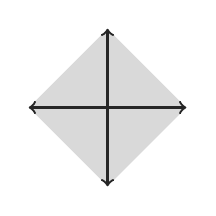
\begin{tikzpicture}
\draw[thick,->] (0,0) -- (0,-1);
\draw[thick,->] (0,0) -- (0,1);
\draw[thick,->] (0,0) -- (-1,0);
\draw[thick,->] (0,0) -- (1,0);

 \path[fill=gray, opacity=0.3] (0, 1) coordinate(p1) --  (-1, 0) coordinate(p2)
 -- (0, -1) coordinate(p3) --
 (1,0) coordinate(p4);
\end{tikzpicture}

\end{document}